% Use only LaTeX2e, calling the article.cls class and 12-point type.

\documentclass[6pt]{rspublic}

% Users of the {thebibliography} environment or BibTeX should use the
% scicite.sty package, downloadable from *Science* at
% www.sciencemag.org/about/authors/prep/TeX_help/ .
% This package should properly format in-text
% reference calls and reference-list numbers.

\usepackage{scicite}

% Use times if you have the font installed; otherwise, comment out the
% following line.

\usepackage{times}

% The preamble here sets up a lot of new/revised commands and
% environments.  It's annoying, but please do *not* try to strip these
% out into a separate .sty file (which could lead to the loss of some
% information when we convert the file to other formats).  Instead, keep
% them in the preamble of your main LaTeX source file.


% The following parameters seem to provide a reasonable page setup.

\topmargin 0.0cm
\oddsidemargin 0.2cm
\textwidth 16cm
\textheight 21cm
\footskip 1.0cm


\usepackage{amsfonts}
\usepackage{graphicx}
\usepackage{epsfig}
\usepackage{epsf}
\usepackage{amssymb}
\usepackage{amsmath}
\usepackage{amsthm}
\usepackage{multirow}


\renewcommand\thefigure{S\arabic{figure}}

\newcommand{\be}{\begin{equation}}
\newcommand{\ee}{\end{equation}}
\newcommand{\bea}{\begin{eqnarray}}
\newcommand{\eea}{\end{eqnarray}}
\newcommand{\Fig}[1]{Fig.\,\ref{#1}}
\newcommand{\Eq}[1]{Eq.\,(\ref{#1})}
\newcommand{\la}{\langle}
\newcommand{\ra}{\rangle}
\newcommand{\nl}{\nonumber \\}
%The next command sets up an environment for the abstract to your paper.

\newenvironment{sciabstract}{%
\begin{quote} \bf}
{\end{quote}}


% If your reference list includes text notes as well as references,
% include the following line; otherwise, comment it out.

%\renewcommand\refname{References and Notes}

% The following lines set up an environment for the last note in the
% reference list, which commonly includes acknowledgments of funding,
% help, etc.  It's intended for users of BibTeX or the {thebibliography}
% environment.  Users who are hand-coding their references at the end
% using a list environment such as {enumerate} can simply add another
% item at the end, and it will be numbered automatically.

\newcounter{lastnote}
\newenvironment{scilastnote}{%
\setcounter{lastnote}{\value{enumiv}}%
\addtocounter{lastnote}{+1}%
\begin{list}%
{\arabic{lastnote}.}
{\setlength{\leftmargin}{.22in}}
{\setlength{\labelsep}{.5em}}}
{\end{list}}


% Include your paper's title here





%%%%%%%%%%%%%%%%% END OF PREAMBLE %%%%%%%%%%%%%%%%



\begin{document}

% Double-space the manuscript.

\baselineskip14pt

% Make the title.





% Place your abstract within the special {sciabstract} environment.



\section*{Supplementary Information}


\subsection*{PPS preparation}

For establishing 4-body spin correlations, which is contained in the form of the PPS, it usually needs multiple pulses and gradient fields in the original spatial average technique. However, in our experiments, we can utilize the GRAPE algorithm not only to calculate shape pulses, but also to seek for a unitary operator, after adding which and a gradient pulse the thermal equilibrium state would transform to the PPS. The initial thermal equilibrium state of the NMR sample can be written as $\rho_{eq}=\sum\limits_{i=1}^4 \gamma_i I_z^i$, where $\gamma_i$ is the gyromagnetic ratio of the nuclear spins. Typically, for the same nuclear spin the value of $\gamma$ can be considered as a unit. The theoretical final state we want to prepare is
\begin{equation}\label{ppsform}
\rho_{theo}=-\frac{1}{16}\mathbb{{I}}+\left\vert 0000 \right\rangle \left\langle0000\right\vert,
\end{equation}
where ${\mathbb{{I}}}$ is the $16\times16$ unity matrix. We will give an initial guess of the unitary operator $U_0$, and calculate the fidelity $F$ between $\rho_{theo}$ and the final state
\begin{equation}\label{ppsform}
\rho_{fin}=Gz(U_0\rho_{eq}U_0^{\dagger}),
\end{equation}
where $Gz$ is a gradient pulse to destroy the coherence (Noting that some coherence like 0-order coherence cannot be destroyed). If $F$ is higher than our pre-set value, specifically 0.99 for this experiment, we will pack $U_0$ into a shape pulse, i.e., GRAPE pulse. Otherwise, we will obtain a new unitary operator $U_1$ through perturbation under the supervision of the GRAPE algorithm, and calculate a new  $F$ by repeating the above procedure. This is the core of our method to prepare the PPS. It needs only one GRAPE pulse and one gradient field, but results a high fidelity PPS.


\begin{figure}[h]
\centering
\begin{minipage}[c]{.6\textwidth}
\centering
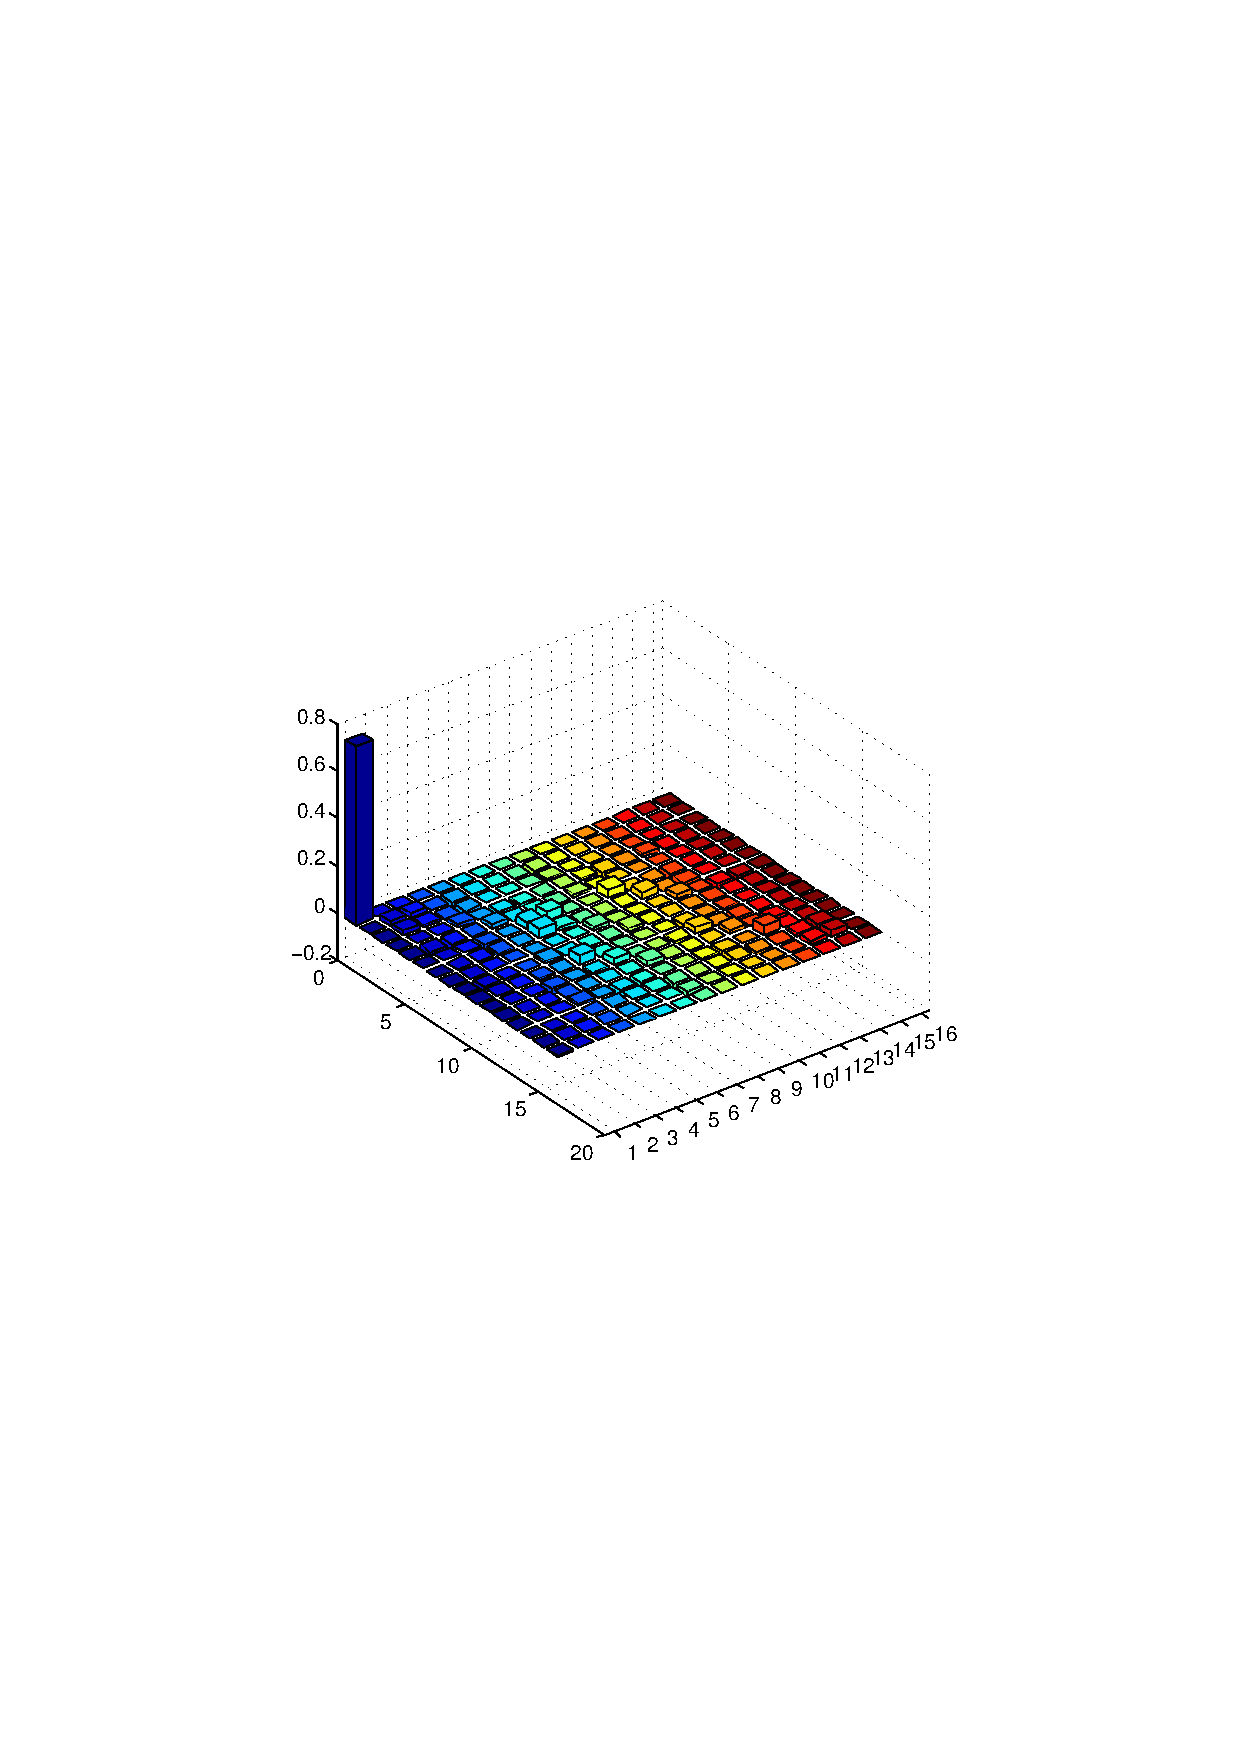
\includegraphics[width=\textwidth]{bar.pdf}
\end{minipage}%
\hspace{.05\textwidth}
\begin{minipage}[c]{.3\textwidth}
\centering
\caption{\footnotesize{Real part of the prepared PPS. After applying the sought unitary operator and a gradient pulse to the thermal equilibrium state, we will obtain the final state which is very similar to $\left\vert 0000 \right\rangle$ if ignoring the identity matrix, which has no influence on the NMR signals. From this figure it can be seen that almost all the signals are concentrated on the population of  $\left\vert 0000 \right\rangle \left\langle 0000 \right\vert$, the peak of which is used as the benchmark of the other measurements of the experiment.}}
\label{pps}
\end{minipage}
\end{figure}


For the sample 1-Bromo-2-Chlorobenzene (C$_6$H$_4$ClBr) in this experiment, with ignoring the off-diagonal elements that cannot be destroyed by the gradient pulse which are close to 0, the diagonal elements of the PPS is [1.512, -0.098,-0.120,-0.109,-0.100,-0.072,-0.112,-0.098,-0.106,-0.136,-0.083,0.097,-0.052,-0.112,-0.081,-0.136].
%\begin{eqnarray}\label{Transformation}
%\left( {\begin{array}{*{20}c}
% {1.512} & {-0.098} & {-0.120} & {-0.109} & {-0.100} & {-0.072} & {-0.112} & {-0.098} \\  \nonumber
% {-0.106} & {-0.136} & {-0.083} & {0.097} & {-0.052} & {-0.112} & {-0.081} & {-0.136} \nonumber
%\end{array}} \right).
%\end{eqnarray}
If deducting the identity matrix from the final state, it is very similar to $\left\vert 0000 \right\rangle$, which indicates that our method is creditable. 







 
 






\end{document}




















